\chapter{Results}\label{chapter:results}

This chapter explains the evaluation methods used for evaluating the performance of machine learning models and presents the results.

\section{Evaluation Criteria} \label{sec:evaluationCriteria}

\subsection{Performance measures}
% Precision, Recall, Fscore
The performance measures \textit{Precision}, \textit{Recall} and \textit{F score} are used for calculating of performance of the machine learning models \textit{SSModel} and \textit{DSModel}.

For the task of protein-location relation extraction, a positive prediction is the one in which the machine learning model predicts a PL (protein-location) relation between a protein entity and a location entity. Similarly, a negative prediction is the one in which the machine learning model predicts that there is no relation between a protein entity and a location entity. 

A prediction can be classified into one of the following categories:


\begin{itemize}

\item \textit{True positive (tp)}: A prediction is said to be a true positive if it is a positive prediction (i.e., the entities are predicted to be related) and it matches an original relation in the corpus.

\item \textit{True negative (tn)}: A prediction is said to be a true negative if it is a negative prediction and the entities in the relation are also not related in the original corpus.

\item \textit{False positive (fp)}: A prediction is said to be a false positive if it is a positive prediction but the participating entities are not related in the original corpus.

\item \textit{False negative (fn)}: A prediction is said to be a false negative if it is a negative prediction but the participating entities are related in the original corpus.

\end{itemize}

\subsubsection*{\textit{Precision}}

Precision is the fraction of true predictions from all predictions and is given by:

$$
\textit{Precision} = \frac{tp}{tp+fp}
$$


\subsubsection*{\textit{Recall}}

Recall is the fraction of true predictions compared to original relations and is given by:

$$
\textit{Recall} = \frac{tp}{tp+fn}
$$

\subsubsection*{\textit{F score}}

F score, also called as F1 score, is the harmonic mean of precision and recall. It is given by:

$$
\textit{F score} = 2 * \frac{Precision * Recall}{Precision + Recall}
$$


\subsection{Evaluation mode - Non unique evaluation} \label{subsec:UniqNonUniqEval}

For a particular document in the corpus, it may happen that a protein is related to a location twice in the document at different places. In the non-unique evaluation mode, such repetitions are considered separately. A predicted relation is said to match with an original relation if and only if the text offsets of both protein and location entities in the predicted relation matches exactly with the text offsets of protein and location entities in the original relation respectively.


% Talk about unique relations here
\subsection{Evaluation mode -  Unique evaluation}

In the unique evaluation mode, a list of unique protein-location relations is made for every document in the corpus, notwithstanding the repetition of relations in the document. A predicted positive relation is said to match if and only if the predicted relation for the document is found in the list of unique relations for that document. If the predicted relation is not found in the list, it is either classified as a false positive or a true negative depending on whether it is a positive prediction or a negative prediction.

\section{Results for \textit{SSModel}}

This section presents the results for same sentence model (\textit{SSModel}). The results are initially discussed for the model trained on training data and evaluated on development data. All experimentation such as feature selection, hyperparameter search is performed with the development data. Once the the number of features to keep and the hyperparameter is fixed, the training model is used to evaluate the test data. The results on unseen test data are considered final results. All following subsections until subsection \ref{subsec:SSFinalRes} presents the results for a model trained on training data and evaluated on development data.

%After all experimentation, an additional model is training combining training and development data. Such a model is used to evaluate the test data and the results in such a way are considered much more robust.
 
\subsection{Initial results}

\begin{figure}
\centering
\begin{minipage}{.5\textwidth}
  \centering
  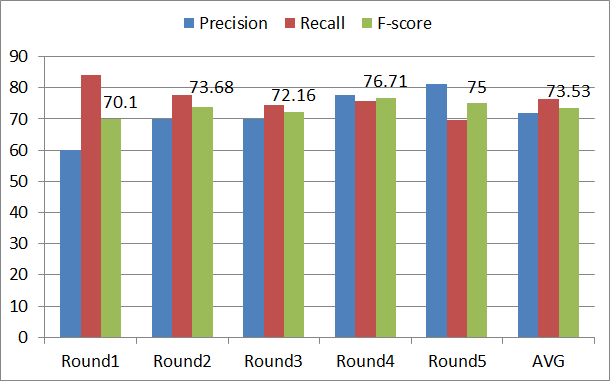
\includegraphics[width=.95\textwidth]{figures/SSInitialResultsNUniq.png}
  \caption{\textit{SSModel} non unique results}
  \label{fig:SS_NU_Initial}
\end{minipage}%
\begin{minipage}{.5\textwidth}
  \centering
  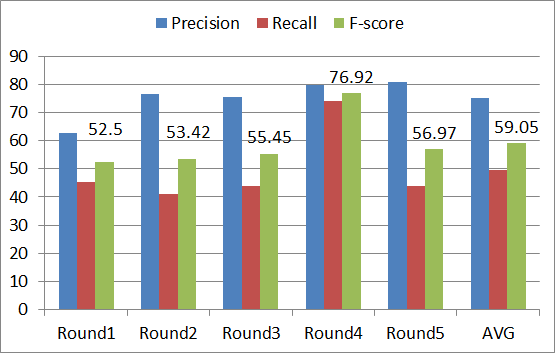
\includegraphics[width=.95\textwidth]{figures/SSInitialResultsUniq.png}
  \caption{\textit{SSModel} unique results}
  \label{fig:SS_U_Initial}
\end{minipage}
\end{figure}

As explained in the section \ref{sec:training}, 5-fold cross-validation is performed on the LocText corpus. For the details of cross-validation, refer to the section \ref{sec:training}. The primary evaluation results are shown in figures \ref{fig:SS_NU_Initial} and \ref{fig:SS_U_Initial}. Figure \ref{fig:SS_NU_Initial} shows the results of \textit{SSModel} using non unique evaluation method and fig. \ref{fig:SS_U_Initial} shows the results of \textit{SSModel} using unique evaluation method. The results are shown in terms of \textit{Precision}, \textit{Recall} and \textit{F score} for every round of cross validation and average performance is shown in the end. The \textit{F score} bars in the figures are also labeled with the actual value. Therefore, the non unique average \textit{F score} for \textit{SSModel} is 73.53 and unique average \textit{F score} for \textit{SSModel} is 59.05 as shown in the figures.

\subsubsection{Experimentation}

In order to make \textit{SSModel} robust and adaptable to other corpus, a lot of experimentation is carried out. Before the experimentation, every round of cross validation creates a model from around 30000 features on average. A lot of these features can be very specific to the LocText corpus and therefore, the efforts are made to discard unnecessary and redundant features. Following types of experiments are carried out:

\begin{itemize}

\item Leave One Out Analysis

\item Feature Weight Ranking

\item Information Gain Analysis

\end{itemize}

These experimentation methods are discussed in upcoming sections. This experimentation falls into the category of feature selection broadly discussed in the section \ref{sec:featSel}.

\subsection{Results after Leave One Out Analysis}

\begin{figure}
\centering
\begin{minipage}{.5\textwidth}
  \centering
  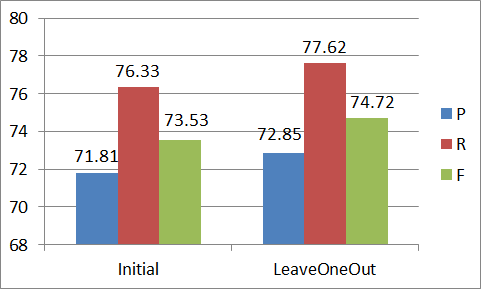
\includegraphics[width=.95\textwidth]{figures/LeaveOneOutNUniq.png}
  \caption{Non unique results comparison}
  \label{fig:LeaveOO_NU}
\end{minipage}%
\begin{minipage}{.5\textwidth}
  \centering
  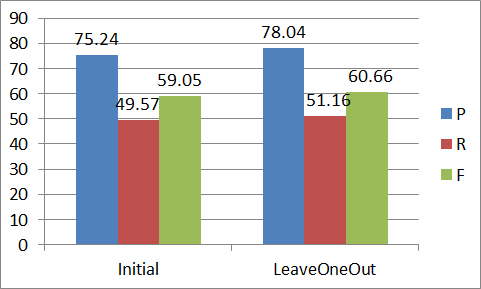
\includegraphics[width=.95\textwidth]{figures/LeaveOneOutUniq.png}
  \caption{Unique results comparison}
  \label{fig:LeaveOO_U}
\end{minipage}
\end{figure}

The theory behind Leave One Out approach is discussed in detail in the subsection \ref{subsec:LeaveOneOut}. To summarize this approach, the feature generators or functions that generates the features are greedily discarded to improve the performance of the model.

Figure \ref{fig:LeaveOO_NU} and \ref{fig:LeaveOO_U} shows the comparison between the results of initial model and after performing the LeaveOneOut experimentation.  The \textit{Precision}, \textit{Recall} and \textit{F score} are denoted by P, R and F respectively. Figure \ref{fig:LeaveOO_NU} shows the comparison using non-unique evaluation method and \ref{fig:LeaveOO_U} shows the comparison using unique evaluation mode. As shown in the figures, the average \textit{F score} increased from 73.53 to 74.72 for non-unique evaluation and from 59.05 to 60.66 for unique evaluation. In addition to the increase in the performance, the initial model used around 30900 features on average in every round of the cross validation. However, the model refined after LeaveOneOut experimentation uses 29000 features on average in every round, therefore reducing the number of features by 1900 for every round of the cross-validation.

\subsection{Results after Feature Weight Ranking}

The Feature Weight Ranking approach, discussed in detail in the subsection \ref{subsec:FWR}, uses the weights of the features for feature selection. The support vector machine model learns the weights for the features. These weights can be extracted from the learned model using a perl script \cite{svmlightonline}. 


\begin{figure}
\centering
\begin{minipage}{.5\textwidth}
  \centering
  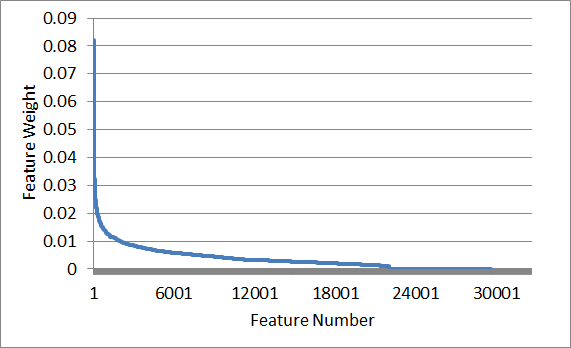
\includegraphics[width=.95\textwidth]{figures/FWRWeightDist.png}
  \caption{Feature weight distribution}
  \label{fig:FWRWeightDist}
\end{minipage}%
\begin{minipage}{.5\textwidth}
  \centering
  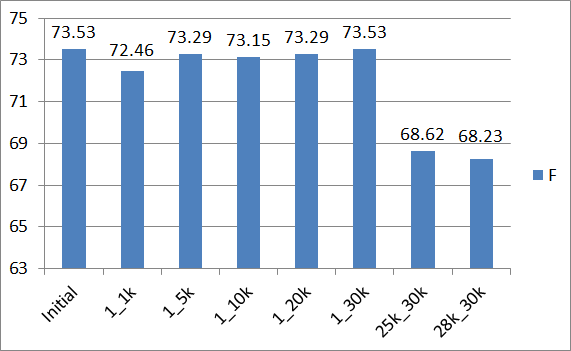
\includegraphics[width=.95\textwidth]{figures/FWRPerformance.png}
  \caption{FWR Performance comparison}
  \label{fig:FWRPerfComp}
\end{minipage}
\end{figure} 

For each round of cross-validation, a model is learned and therefore, the feature weights can be extracted for every round. Figure \ref{fig:FWRWeightDist} shows the distribution of weights for features of round 1. The distribution of feature weights in other folds follow similar distribution. As shown in the figure, there are very less features with higher weights and most of the features have comparatively lower weights. In addition, none of the features have a drastically low weight which implies that every feature has some or other information.

Figure \ref{fig:FWRPerfComp} shows the comparison of performance of various FWR models with initial model. Only average \textit{F scores} are shown for comparison. The model \textit{1\_1k} implies that 1000 highest weighted features are selected from every round of cross validation and the model is trained using only those features. Similar terminology applies for rest of the FWR models shown in the figure. None of the FWR models have a higher performance than the initial model. The performance of FWR model with first 1000 features (\textit{1\_1k}) is lower than FWR model with first 5000 features (\textit{1\_5k}). It is also seen that the performance drops for first 20000 features and then again increases for first 30000 features. This trend invalidates the intuition that higher weighted features should result in higher performance and addition of lower weighted features should decrease the performance. In our case, addition of features ranked 20000 to 30000 have actually increased the performance. The FWR model consisiting of lowest 2000 features in every round (\textit{28k\_30k}) also has considerable performance and cannot be discarded as useless. Owing to all these problems, this approach was not carried forward.
 
\subsection{Results after Information Gain Analysis}

Information gain is widely used technique for the purpose of feature selection. The theoretical background for calculating information gain can be found in subsection \ref{subsec:IG}. The information gain is calculated for features in every round of cross validation and analysis is done similar to the analysis based on feature weights.

\begin{figure}
\centering
\begin{minipage}{.5\textwidth}
  \centering
  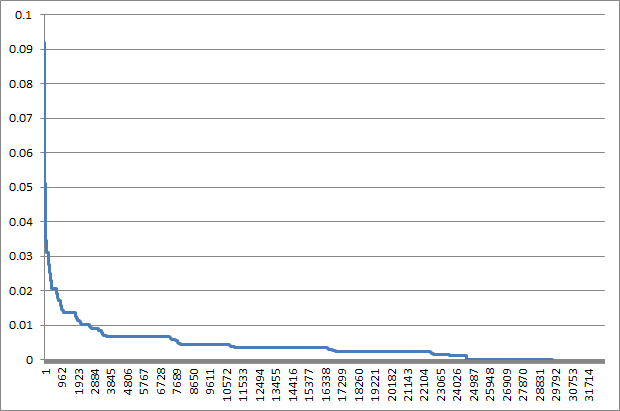
\includegraphics[width=.95\textwidth]{figures/IGDistr1.png}
  \caption{Information Gain distribution}
  \label{fig:IGDist}
\end{minipage}%
\begin{minipage}{.5\textwidth}
  \centering
  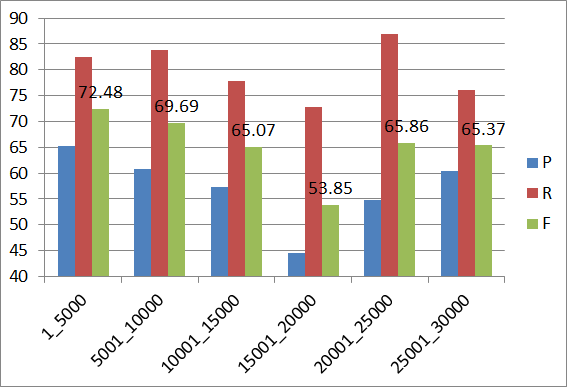
\includegraphics[width=.95\textwidth]{figures/IG5kSlabsComp.png}
  \caption{IG models with 5k slabs}
  \label{fig:IG5kComp}
\end{minipage}
\end{figure} 

Figure \ref{fig:IGDist} shows the information gain of features used in round 1. The distribution of information gain is similar to the distribution of feature weights with minor difference that the feature weight distribution is much smoother than the distribution of information gain. To analyze the effectiveness of features with different information gain, an experiment was conducted by dividing the features into slabs of 5000 features depending on their information gain. Figure \ref{fig:IG5kComp} shows the average performance of various models trained with slabs of 5000 features. The model \textit{1\_5000} uses the first 5000 features with best information gain, the model \textit{5001\_10000} uses next 5000 features and so on. As can be seen in the figure, none of the 5k models have exceptionally low performance except model \textit{15001\_20000}. This further consolidates the finding of \cite{joachims1998text} that all features have some or other information and aggressive feature selection might not result in manifold increase in the performance.

Further experiments were carried out using some of the features with best information gain. For this purpose, first 5000 features were considered. Different models were trained using first 1000, 2000, 4000 and 5000 features and their performance was compared with the initial model.  Figure \ref{fig:IG_5k_NU} shows the comparison of models using non unique evaluation method and \ref{fig:IG_5k_U} shows the comparison of models using unique evaluation method. As seen in the fig. \ref{fig:IG_5k_U}, the model with first 2000 features registers much better performance than the initial model. For the same model, the non unique comparison shows highest increase in the \textit{Recall}. Therefore, it was decided to investigate the model with first 2000 features further.

\begin{figure}
\centering
\begin{minipage}{.5\textwidth}
  \centering
  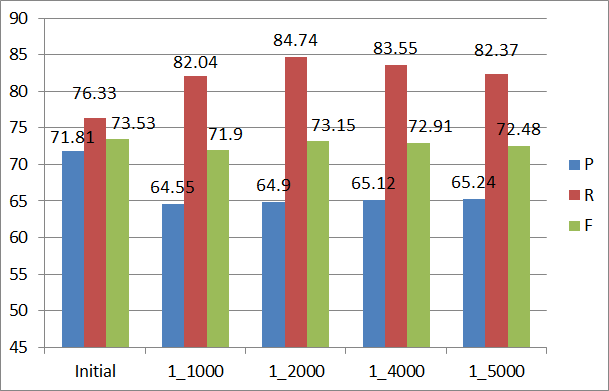
\includegraphics[width=.95\textwidth]{figures/IGFirst5k_NU.png}
  \caption{IG non unique comparison}
  \label{fig:IG_5k_NU}
\end{minipage}%
\begin{minipage}{.5\textwidth}
  \centering
  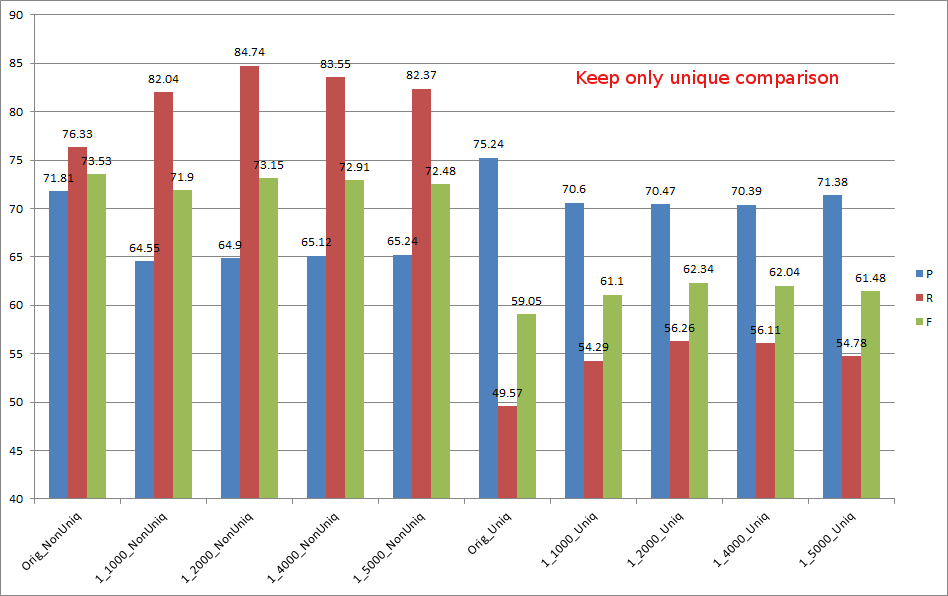
\includegraphics[width=.95\textwidth]{figures/IGFirst5k_U.png}
  \caption{IG unique comparison}
  \label{fig:IG_5k_U}
\end{minipage}
\end{figure} 


As described previously, the features are generated by feature generators or functions. Note that the term feature generator and feature functions mean the same and used interchangeably in the explanation ahead. In order to discard bad features, the solution is to discard the feature generators. A feature generator can generate a lot of features and the options is to either keep all of them or discard all of them. Hence, it was necessary to trace back the feature generators that generates these 2000 features with best information gain. Once the feature generators are located, other features generators can be discarded and the performance of such a model can be observed.

To trace back the feature generators, every feature was given a label indicating the feature generator that produced it. There were a total of 109 feature generators and to choose some of them, it was necessary to assign a statistic to each feature generator. Following criteria were used for selection of feature generators:

\begin{itemize}

\item \textbf{Total information gain:} For every feature generator, the information gain of its features in all 5 rounds of cross validation was summed up to produce a number called total information gain.

\item \textbf{Number of features:} The number of features produced by each feature generator.

\item \textbf{Average information gain:} Average information gain for a feature generator was calculated by dividing total information gain by number of features produced by it.

\item \textbf{Minimum information gain:} Minimum information gain for a feature generator is equal to minimum of information gains of its features.

\item \textbf{Maximum information gain:} Maximum information gain for a feature generator is equal to maximum of information gains of its features.

\end{itemize}

Using these 5 statistics, an exhaustive search was conducted to select the best model. For every statistic, a model was trained and evaluated using some or all of the feature generators. For example, if the statistic total information gain is considered, 109 models were trained and evaluated. The models were named as TIG\_1 to TIG\_109. TIG\_1 implies that the criteria total information gain (TIG) is used to choose a single feature generator with best total information gain. Similarly, TIG\_10 indicates a model where 10 feature generators having best total information gain were chosen and the model was trained. Such experiments were conducted for all of the 5 criteria/statistics mentioned above. Some of the interesting results are explained in the figures \ref{fig:AvgIG} and \ref{fig:MinIG}.

\begin{figure}
\centering
\begin{minipage}{.5\textwidth}
  \centering
  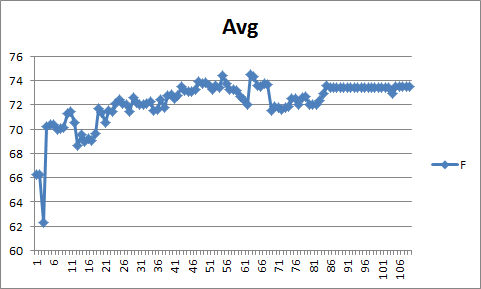
\includegraphics[width=.95\textwidth]{figures/AvgIGAnalysis.png}
  \caption{Average IG experiments}
  \label{fig:AvgIG}
\end{minipage}%
\begin{minipage}{.5\textwidth}
  \centering
  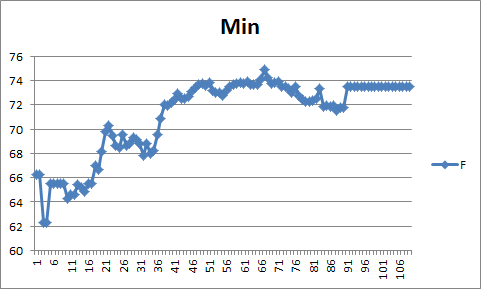
\includegraphics[width=.95\textwidth]{figures/MinIGAnalysis.png}
  \caption{Minimum IG experiments}
  \label{fig:MinIG}
\end{minipage}
\end{figure} 

Figures \ref{fig:AvgIG} and \ref{fig:MinIG} shows the variation of \textit{F scores} of different models created using average information gain and minimum information gain respectively. The last point in the line graph Avg\_109 or Min\_109 indicates the performance of model using all 109 feature generator or in other words without any feature selection. The performance of Avg\_109 and Min\_109, therefore, is equal to the performance of initial model which is a \textit{F score} of 73.53 according to non unique evaluation method. In figure \ref{fig:AvgIG}, there are 3 models, viz., Avg\_55, Avg\_63 and Avg\_64 that have better performance than the initial model (Avg\_109). Similarly, in the figure \ref{fig:MinIG}, there are 3 points, viz., Min\_66, Min\_67 and Min\_68 that have better performance than the initial model (Min\_109). These 6 models were selected and analyzed.

\begin{figure}
\centering
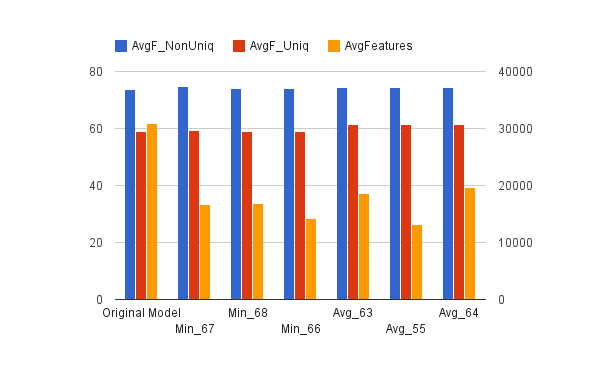
\includegraphics[scale=0.6]{figures/6ModelsComparison.png}
\caption{Comparison of selected models with initial model}\label{fig:6ModelsComp}
\end{figure}

As shown in the fig. \ref{fig:6ModelsComp}, Avg\_55 has near to best performance with respect to non unique evaluation mode, best performance with respect to unique evaluation mode and highest reduction in the number of features. The average number of feature for Avg\_55 is around 13230 compared to 30900 in the initial model. Therefore, Avg\_55 models was selected as the best \textit{SSModel}.


\subsection{Hyperparameter search results}

Exhaustive hyperparameter search was conducted for the selected model Avg\_55. The hyperparameter for support vector machine model is the regularization parameter $\mathbf{C}$ which determines the trade-off between training error and margin as explained in the section \ref{subsec:RegPar}. Experiments were conducted for finding the best regularization parameter by varying $\mathbf{C}$ from 0.0000 to 2.0000 with the steps of 0.0005. A value of 0.0005 was found to be the best hyperparameter value which results in increase in performance of 1.76 with respect to unique evaluation mode. The hyperparameter search was done to  maximize the performance with respect to unique evaluation mode.

\begin{figure}
\centering
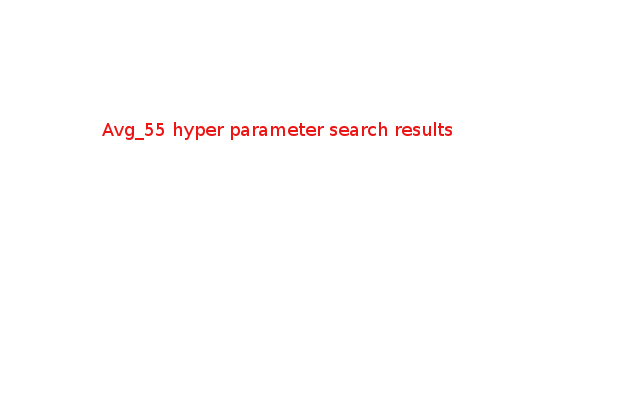
\includegraphics[scale=0.6]{figures/SSModelRegPar.png}
\caption{Results before and after hyperparameter search}\label{fig:SSModelRegPar}
\end{figure}

\subsection{Final Results}\label{subsec:SSFinalRes}

\section{Results for \textit{DSModel}}

\section{Results for CombinedModel}

\section{Assessment of Performance evaluation results}

%  Explain about statistical significance tests